\subsubsection{Expense Management}
\label{sec:expense-management}

This functional area encompasses all features related to expense management. It includes functionalities such as uploading, editing, and deleting expenses, as well as obtaining AI-extracted data and assigning expenses to either a new or an existing report. All these actions are accessible within the Expenses List page view, as shown in Figure \ref{fig:expense-management-use-case-diagram}.

\begin{figure}[H]
    \centering
    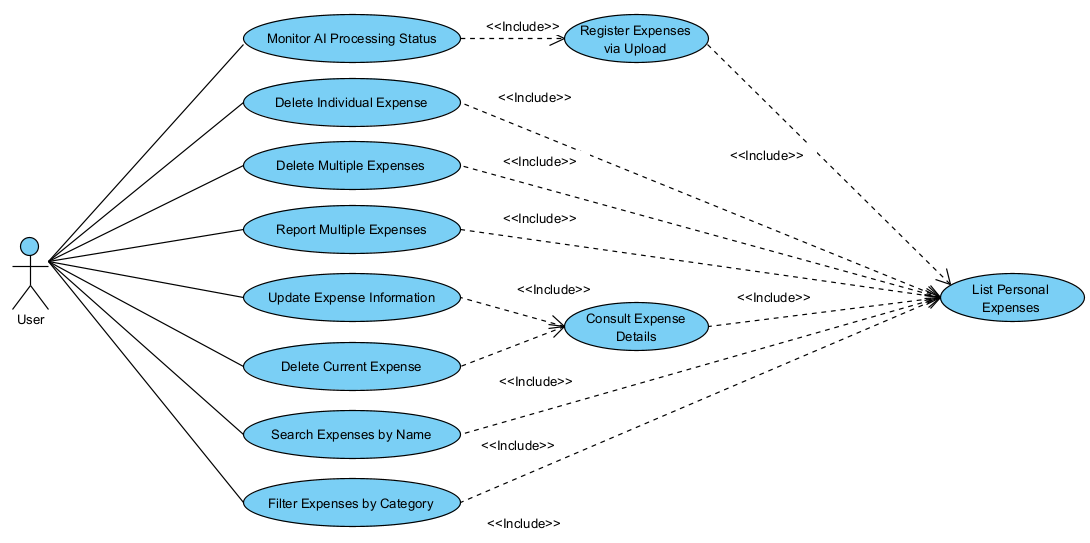
\includegraphics[width=\textwidth]{Images/expensemanagement.png}
    \caption[Expense management use case diagram]
    {Expense management use case diagram. [Own creation]}
    \label{fig:expense-management-use-case-diagram}
\end{figure}

\textbf{Use Case: Register Expenses via Upload}

\textbf{Primary Actor:} User

\textbf{Trigger:} The user uploads or drops one or more receipts.

\textbf{Preconditions:} The user is successfully authenticated and viewing the Expenses page.

\textbf{Postconditions:} The new expenses are successfully registered and added to the AI processing queue.

\vspace{0.5cm}

\textbf{Main Success Scenario:}

\begin{enumerate}[leftmargin=0.75cm, noitemsep]
    \item The user uploads or drops one or more receipts.
    \item The system registers new expense records, associates them with the authenticated user, and queues them for automated data extraction.
    \item The system updates the expense list to include the recently uploaded items.
\end{enumerate}

\vspace{0.3cm}

\textbf{Extensions:}

\begin{itemize}[label={}, leftmargin=0.75cm, noitemsep]
    \item \textbf{2a. Invalid File Format:}
    \begin{itemize}[label={}, leftmargin=0.75cm, noitemsep]
        \item 2a1. The system detects that the uploaded file format is not supported (non-image or non-PDF).
        \item 2a2. The system rejects the upload and keeps the user on the current page without registering any expense.
    \end{itemize}

    \item \textbf{2b. Database Connection Error:}
    \begin{itemize}[label={}, leftmargin=0.75cm, noitemsep]
        \item 2b1. The system is unable to register the expense records due to a database connection failure.
        \item 2b2. The system notifies the user of the error and no expenses are registered.
    \end{itemize}
\end{itemize}